\documentclass[a4paper,11pt]{article}

\usepackage{../préambule}

\begin{luacode}
	function myAdd(x, y)
		tex.sprint(x + y)
	end
\end{luacode}

\makeatletter
\renewcommand{\maketitle}{%
{\scriptsize colle dans ton cahier d'exercices, et écrit dans ton cahier} \vspace{0.5em}

	\begin{center}
		\LARGE
		\myuline{\@title}
		\vspace{1em}
	\end{center}
}
\makeatother

\title{Activité : mesurer le temps}
\date{}
\author{}

\begin{document}

\maketitle

\section{Cadrans solaires}

\begin{greybox}[frametitle={Point historique}]
	Les \textbf{cadrans solaires} sont des outils pour mesurer le temps. Leur première apparition date d'il y a environ 2400 ans !
\end{greybox}

\begin{attention}[frametitle={Comment ça fonctionne ?}]
	\begin{center}
		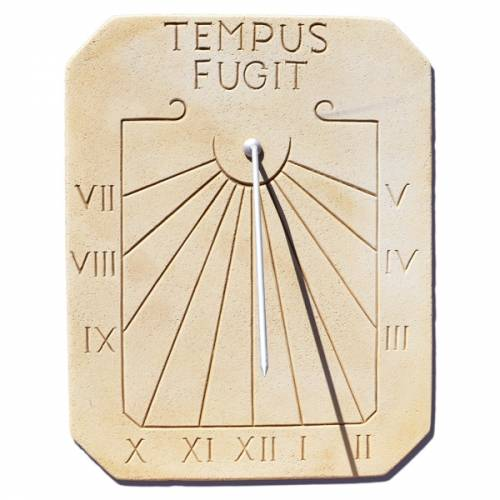
\includegraphics[width=0.2\linewidth]{Images/cadran solaire.jpeg}
	\end{center}

	Lorsqu'il y a du soleil, l'aiguille fait de l'ombre sur le cadran : cette ombre indique l'heure qu'il est.
\end{attention}

{\small \begin{vocabulaire}[Schéma]
	Un \textbf{schéma} est une représentation simpifiée d'un objet.
\end{vocabulaire}}

On a schématisé un cadran solaire ci dessous: \vspace{1em}

\begin{center}
	\begin{tikzpicture}[scale=0.95]
		\draw (4,0) arc(0:-180:4cm);

		\draw[ultra thick,|-] (0,0) -- (0,-1.8);
		\draw[thick,rotate around={56.25:(0,0)}] (0,0) -- (-4.2,0);

		\node at (1,-1) {\footnotesize ← Aiguille};
		\node at (-1.5,-0.7) {\footnotesize Ombre →};

		\draw (4,0) -- (3,0);
		\foreach \angle in {-15,-30,-45,-60,-75,-90,-105,-120,-135,-150,-165,-180} {
				\draw[rotate around={\angle:(0,0)}] (4,0) -- (3,0);
				\draw[rotate around={\directlua{myAdd(\angle, 7.5)}:(0,0)}] (4,0) -- (3.5,0);
			}
	\end{tikzpicture}
\end{center} \vspace{1.5em}

\begin{enumerate}
	\item Compte le nombre de grandes graduations : à quoi correspondent-elles ? (rappelles-toi que le cadran solaire ne fonctionne que de jour). \vspace{0.5em}

	      ........................................................................................................................
	\item Là où ce cadran est placé, le soleil se lève à droite du cadran à 8 heures, et se couche à gauche du cadran à 20 heures.

	      Indique sur le schéma les heures de la journée.
	\item À quoi correspondent les petites graduations ? \vspace{0.5em}

	      ........................................................................................................................
	\item Quelle heure est indiquée sur ce cadran ? Précise les minutes. \vspace{0.5em}

	      ........................................................................................................................
\end{enumerate}

\newpage

\section{L'horloge mécanique et la montre à ressort}

\begin{greybox}[frametitle={Point historique}]
	L'horloge mécanique a été inventée vers le 14\textsuperscript{ème} siècle, la montre à ressort au 16\textsuperscript{ème} siècle.
\end{greybox}

\begin{attention}[frametitle={Comment ça fonctionne ?}]
	\begin{center}
		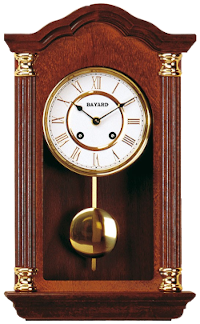
\includegraphics[width=0.2\linewidth]{Images/horloge mécanique.png}
		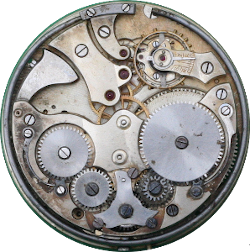
\includegraphics[width=0.3\linewidth]{Images/montre mécanique.png}
	\end{center}

	Le pendule de l'horloge, ou le ressort de la montre, fait tourner un rouage à chaque battement.
\end{attention}

On a une montre à ressort, dans laquelle il y a 3 rouages.
\begin{itemize}
	\item Chaque rouage fait avancer le prochain d'une cran lorsqu'il finit un tour complet.
	\item Le premier rouage tourne d'un cran à chaque vibration du ressort.
	\item Lorque le 2\textsuperscript{ème} rouage fait un tour complet, l'aiguille des secondes avance d'un cran.
	\item Lorque le 3\textsuperscript{ème} rouage fait un tour complet, l'aiguille des minutes avance d'un cran.
\end{itemize}
\squared{\textbf{Questions :}}
\begin{enumerate}
	\item Combien y-a-t'il de crans sur le troisième rouage ? .......................................
	\item Supposons que le premier rouage a 10 crans, et le deuxième en a 32.

	      Combien faut-il de vibrations du ressort pour faire avancer l'aiguille des secondes ? \vspace{0.5em}

	      ....................................................................................................................... \vspace{0.5em}

	\item Tous les combien de temps le ressort vibre-il ? ..............................................
\end{enumerate}

\newpage

\section{L'horloge atomique}

\begin{greybox}[frametitle={Point historique}]
	La première horloge atomique a été inventée en 1948. Elles sont aujourd'hui utilisée lorqu'on a besoin de mesurer très précisément le temps (c'est-à-dire souvent !).
\end{greybox}

\begin{attention}[frametitle={Comment ça fonctionne ?}]
	La plupart de ces horloges utilisent du \textbf{césium}, un type de métal.

	Le césium bouge (il "oscille") de manière régulière : \squared{9 192 631 770} fois \textbf{par seconde} ! L'horloge compte donc ces mouvements pour suivre l'évolution du temps, et fonctionne ensuite de manière similaire à une horloge mécanique.
\end{attention}

\begin{enumerate}
	\item Le nombre de d'oscillations du césium est-il proportionnel au temps en secondes ? \vspace{0.6em}

	      ........................................................................................................................

	      Est-il proportionnel au temps en minutes ? Quel est le coefficient de proportionnalité ? \vspace{0.6em}

	      ........................................................................................................................
	\item Une horloge atomique se trompe de temps en temps : une très bonne horloge gagne $\frac{1}{10^{13}}$ seconde de décalage \textbf{chaque seconde} ($10^{13} = $ un 1 suivi de 13 zéros).

	      Au bout de combien d'années une telle horloge aura-elle gagné 1 seconde de décalage ? \vspace{0.6em}

	      ........................................................................................................................
\end{enumerate}

\end{document}